


\tikzset{every picture/.style={line width=0.75pt}} %set default line width to 0.75pt        

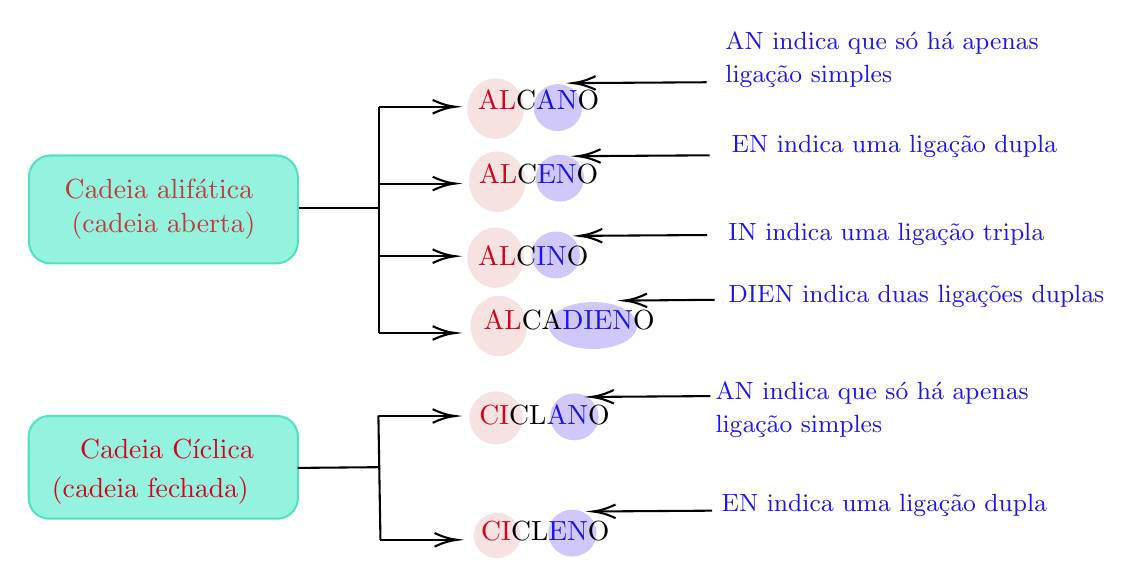
\begin{tikzpicture}[x=0.75pt,y=0.75pt,yscale=-1,xscale=1]
	%uncomment if require: \path (0,322); %set diagram left start at 0, and has height of 322
	
	%Rounded Rect [id:dp08223711771224063] 
	\draw  [color={rgb, 255:red, 80; green, 227; blue, 194 }  ,draw opacity=1 ][fill={rgb, 255:red, 148; green, 243; blue, 222 }  ,fill opacity=1 ] (61.13,74.87) .. controls (61.13,69.12) and (65.79,64.47) .. (71.53,64.47) -- (180.27,64.47) .. controls (186.01,64.47) and (190.67,69.12) .. (190.67,74.87) -- (190.67,106.07) .. controls (190.67,111.81) and (186.01,116.47) .. (180.27,116.47) -- (71.53,116.47) .. controls (65.79,116.47) and (61.13,111.81) .. (61.13,106.07) -- cycle ;
	
	%Rounded Rect [id:dp6837192782695966] 
	\draw  [color={rgb, 255:red, 80; green, 227; blue, 194 }  ,draw opacity=1 ][fill={rgb, 255:red, 148; green, 243; blue, 222 }  ,fill opacity=1 ] (61,199.89) .. controls (61,194.43) and (65.43,190) .. (70.89,190) -- (180.77,190) .. controls (186.24,190) and (190.67,194.43) .. (190.67,199.89) -- (190.67,229.57) .. controls (190.67,235.04) and (186.24,239.47) .. (180.77,239.47) -- (70.89,239.47) .. controls (65.43,239.47) and (61,235.04) .. (61,229.57) -- cycle ;
	
	%Straight Lines [id:da6268575897929107] 
	\draw    (191.05,90) -- (216.63,90) -- (229.05,90) ;
	%Straight Lines [id:da3912391218322656] 
	\draw    (190.55,215) -- (229.97,214.65) ;
	%Straight Lines [id:da4298017873828953] 
	\draw    (229.55,41) -- (229.55,150) ;
	%Straight Lines [id:da4620664162425595] 
	\draw    (229.55,41) -- (264.55,41) ;
	\draw [shift={(266.55,41)}, rotate = 180] [color={rgb, 255:red, 0; green, 0; blue, 0 }  ][line width=0.75]    (10.93,-3.29) .. controls (6.95,-1.4) and (3.31,-0.3) .. (0,0) .. controls (3.31,0.3) and (6.95,1.4) .. (10.93,3.29)   ;
	%Straight Lines [id:da6877154695298078] 
	\draw    (229.55,78) -- (264.55,78) ;
	\draw [shift={(266.55,78)}, rotate = 180] [color={rgb, 255:red, 0; green, 0; blue, 0 }  ][line width=0.75]    (10.93,-3.29) .. controls (6.95,-1.4) and (3.31,-0.3) .. (0,0) .. controls (3.31,0.3) and (6.95,1.4) .. (10.93,3.29)   ;
	%Straight Lines [id:da7148044014610523] 
	\draw    (229.55,113) -- (264.55,113) ;
	\draw [shift={(266.55,113)}, rotate = 180] [color={rgb, 255:red, 0; green, 0; blue, 0 }  ][line width=0.75]    (10.93,-3.29) .. controls (6.95,-1.4) and (3.31,-0.3) .. (0,0) .. controls (3.31,0.3) and (6.95,1.4) .. (10.93,3.29)   ;
	%Straight Lines [id:da2252897061575344] 
	\draw    (229.55,150) -- (264.55,150) ;
	\draw [shift={(266.55,150)}, rotate = 180] [color={rgb, 255:red, 0; green, 0; blue, 0 }  ][line width=0.75]    (10.93,-3.29) .. controls (6.95,-1.4) and (3.31,-0.3) .. (0,0) .. controls (3.31,0.3) and (6.95,1.4) .. (10.93,3.29)   ;
	%Shape: Ellipse [id:dp7986791667582457] 
	\draw  [color={rgb, 255:red, 247; green, 226; blue, 226 }  ,draw opacity=1 ][fill={rgb, 255:red, 247; green, 226; blue, 226 }  ,fill opacity=1 ] (272.8,41.9) .. controls (272.8,34.11) and (278.68,27.8) .. (285.93,27.8) .. controls (293.19,27.8) and (299.07,34.11) .. (299.07,41.9) .. controls (299.07,49.69) and (293.19,56) .. (285.93,56) .. controls (278.68,56) and (272.8,49.69) .. (272.8,41.9) -- cycle ;
	%Shape: Ellipse [id:dp6720086785512882] 
	\draw  [color={rgb, 255:red, 247; green, 226; blue, 226 }  ,draw opacity=1 ][fill={rgb, 255:red, 247; green, 226; blue, 226 }  ,fill opacity=1 ] (273.6,77.1) .. controls (273.6,69.31) and (279.48,63) .. (286.73,63) .. controls (293.99,63) and (299.87,69.31) .. (299.87,77.1) .. controls (299.87,84.89) and (293.99,91.2) .. (286.73,91.2) .. controls (279.48,91.2) and (273.6,84.89) .. (273.6,77.1) -- cycle ;
	%Shape: Ellipse [id:dp15012520451579814] 
	\draw  [color={rgb, 255:red, 247; green, 226; blue, 226 }  ,draw opacity=1 ][fill={rgb, 255:red, 247; green, 226; blue, 226 }  ,fill opacity=1 ] (272.8,113.7) .. controls (272.8,105.91) and (278.68,99.6) .. (285.93,99.6) .. controls (293.19,99.6) and (299.07,105.91) .. (299.07,113.7) .. controls (299.07,121.49) and (293.19,127.8) .. (285.93,127.8) .. controls (278.68,127.8) and (272.8,121.49) .. (272.8,113.7) -- cycle ;
	%Shape: Ellipse [id:dp5861118582212286] 
	\draw  [color={rgb, 255:red, 247; green, 226; blue, 226 }  ,draw opacity=1 ][fill={rgb, 255:red, 247; green, 226; blue, 226 }  ,fill opacity=1 ] (274.4,146.7) .. controls (274.4,138.91) and (280.28,132.6) .. (287.53,132.6) .. controls (294.79,132.6) and (300.67,138.91) .. (300.67,146.7) .. controls (300.67,154.49) and (294.79,160.8) .. (287.53,160.8) .. controls (280.28,160.8) and (274.4,154.49) .. (274.4,146.7) -- cycle ;
	%Straight Lines [id:da04862363537332304] 
	\draw    (229.47,189.65) -- (230.47,249.65) ;
	%Straight Lines [id:da5215534876730717] 
	\draw    (229.55,190) -- (264.55,190) ;
	\draw [shift={(266.55,190)}, rotate = 180] [color={rgb, 255:red, 0; green, 0; blue, 0 }  ][line width=0.75]    (10.93,-3.29) .. controls (6.95,-1.4) and (3.31,-0.3) .. (0,0) .. controls (3.31,0.3) and (6.95,1.4) .. (10.93,3.29)   ;
	%Straight Lines [id:da4160518205492374] 
	\draw    (230.47,249.65) -- (265.47,249.65) ;
	\draw [shift={(267.47,249.65)}, rotate = 180] [color={rgb, 255:red, 0; green, 0; blue, 0 }  ][line width=0.75]    (10.93,-3.29) .. controls (6.95,-1.4) and (3.31,-0.3) .. (0,0) .. controls (3.31,0.3) and (6.95,1.4) .. (10.93,3.29)   ;
	%Shape: Ellipse [id:dp4727286644743499] 
	\draw  [color={rgb, 255:red, 247; green, 226; blue, 226 }  ,draw opacity=1 ][fill={rgb, 255:red, 247; green, 226; blue, 226 }  ,fill opacity=1 ] (273.8,190.9) .. controls (273.8,184.11) and (279.32,178.6) .. (286.13,178.6) .. controls (292.94,178.6) and (298.47,184.11) .. (298.47,190.9) .. controls (298.47,197.69) and (292.94,203.2) .. (286.13,203.2) .. controls (279.32,203.2) and (273.8,197.69) .. (273.8,190.9) -- cycle ;
	%Shape: Ellipse [id:dp8716137570866761] 
	\draw  [color={rgb, 255:red, 247; green, 226; blue, 226 }  ,draw opacity=1 ][fill={rgb, 255:red, 247; green, 226; blue, 226 }  ,fill opacity=1 ] (275.87,247.6) .. controls (275.87,241.86) and (280.7,237.2) .. (286.67,237.2) .. controls (292.63,237.2) and (297.47,241.86) .. (297.47,247.6) .. controls (297.47,253.34) and (292.63,258) .. (286.67,258) .. controls (280.7,258) and (275.87,253.34) .. (275.87,247.6) -- cycle ;
	%Shape: Ellipse [id:dp7373775338432144] 
	\draw  [color={rgb, 255:red, 208; green, 200; blue, 250 }  ,draw opacity=1 ][fill={rgb, 255:red, 208; green, 200; blue, 250 }  ,fill opacity=1 ] (304.8,41.4) .. controls (304.8,35.44) and (309.78,30.6) .. (315.93,30.6) .. controls (322.08,30.6) and (327.07,35.44) .. (327.07,41.4) .. controls (327.07,47.36) and (322.08,52.2) .. (315.93,52.2) .. controls (309.78,52.2) and (304.8,47.36) .. (304.8,41.4) -- cycle ;
	%Shape: Ellipse [id:dp7097136496359834] 
	\draw  [color={rgb, 255:red, 208; green, 200; blue, 250 }  ,draw opacity=1 ][fill={rgb, 255:red, 208; green, 200; blue, 250 }  ,fill opacity=1 ] (305.8,75.4) .. controls (305.8,69.44) and (310.78,64.6) .. (316.93,64.6) .. controls (323.08,64.6) and (328.07,69.44) .. (328.07,75.4) .. controls (328.07,81.36) and (323.08,86.2) .. (316.93,86.2) .. controls (310.78,86.2) and (305.8,81.36) .. (305.8,75.4) -- cycle ;
	%Shape: Ellipse [id:dp9114404112334205] 
	\draw  [color={rgb, 255:red, 208; green, 200; blue, 250 }  ,draw opacity=1 ][fill={rgb, 255:red, 208; green, 200; blue, 250 }  ,fill opacity=1 ] (303.8,112.4) .. controls (303.8,106.44) and (308.78,101.6) .. (314.93,101.6) .. controls (321.08,101.6) and (326.07,106.44) .. (326.07,112.4) .. controls (326.07,118.36) and (321.08,123.2) .. (314.93,123.2) .. controls (308.78,123.2) and (303.8,118.36) .. (303.8,112.4) -- cycle ;
	%Shape: Ellipse [id:dp5914650769407996] 
	\draw  [color={rgb, 255:red, 208; green, 200; blue, 250 }  ,draw opacity=1 ][fill={rgb, 255:red, 208; green, 200; blue, 250 }  ,fill opacity=1 ] (312.8,190.4) .. controls (312.8,184.44) and (317.78,179.6) .. (323.93,179.6) .. controls (330.08,179.6) and (335.07,184.44) .. (335.07,190.4) .. controls (335.07,196.36) and (330.08,201.2) .. (323.93,201.2) .. controls (317.78,201.2) and (312.8,196.36) .. (312.8,190.4) -- cycle ;
	%Shape: Ellipse [id:dp6476957834979115] 
	\draw  [color={rgb, 255:red, 208; green, 200; blue, 250 }  ,draw opacity=1 ][fill={rgb, 255:red, 208; green, 200; blue, 250 }  ,fill opacity=1 ] (311.8,246.4) .. controls (311.8,240.44) and (316.78,235.6) .. (322.93,235.6) .. controls (329.08,235.6) and (334.07,240.44) .. (334.07,246.4) .. controls (334.07,252.36) and (329.08,257.2) .. (322.93,257.2) .. controls (316.78,257.2) and (311.8,252.36) .. (311.8,246.4) -- cycle ;
	%Shape: Ellipse [id:dp6542210161459149] 
	\draw  [color={rgb, 255:red, 208; green, 200; blue, 250 }  ,draw opacity=1 ][fill={rgb, 255:red, 208; green, 200; blue, 250 }  ,fill opacity=1 ] (312.07,146.4) .. controls (312.07,140.44) and (321.38,135.6) .. (332.87,135.6) .. controls (344.35,135.6) and (353.67,140.44) .. (353.67,146.4) .. controls (353.67,152.36) and (344.35,157.2) .. (332.87,157.2) .. controls (321.38,157.2) and (312.07,152.36) .. (312.07,146.4) -- cycle ;
	%Straight Lines [id:da04199800870117343] 
	\draw    (387.67,29.2) -- (325.2,29.59) ;
	\draw [shift={(323.2,29.6)}, rotate = 359.64] [color={rgb, 255:red, 0; green, 0; blue, 0 }  ][line width=0.75]    (10.93,-3.29) .. controls (6.95,-1.4) and (3.31,-0.3) .. (0,0) .. controls (3.31,0.3) and (6.95,1.4) .. (10.93,3.29)   ;
	%Straight Lines [id:da8568733656361407] 
	\draw    (389.07,64.4) -- (327.6,64.79) ;
	\draw [shift={(325.6,64.8)}, rotate = 359.64] [color={rgb, 255:red, 0; green, 0; blue, 0 }  ][line width=0.75]    (10.93,-3.29) .. controls (6.95,-1.4) and (3.31,-0.3) .. (0,0) .. controls (3.31,0.3) and (6.95,1.4) .. (10.93,3.29)   ;
	%Straight Lines [id:da9044602404765214] 
	\draw    (389.47,180.4) -- (334,180.79) ;
	\draw [shift={(332,180.8)}, rotate = 359.6] [color={rgb, 255:red, 0; green, 0; blue, 0 }  ][line width=0.75]    (10.93,-3.29) .. controls (6.95,-1.4) and (3.31,-0.3) .. (0,0) .. controls (3.31,0.3) and (6.95,1.4) .. (10.93,3.29)   ;
	%Straight Lines [id:da7022544313414875] 
	\draw    (387.87,102.8) -- (328.4,103.19) ;
	\draw [shift={(326.4,103.2)}, rotate = 359.63] [color={rgb, 255:red, 0; green, 0; blue, 0 }  ][line width=0.75]    (10.93,-3.29) .. controls (6.95,-1.4) and (3.31,-0.3) .. (0,0) .. controls (3.31,0.3) and (6.95,1.4) .. (10.93,3.29)   ;
	%Straight Lines [id:da33632408982471707] 
	\draw    (391.47,134) -- (350,134.38) ;
	\draw [shift={(348,134.4)}, rotate = 359.47] [color={rgb, 255:red, 0; green, 0; blue, 0 }  ][line width=0.75]    (10.93,-3.29) .. controls (6.95,-1.4) and (3.31,-0.3) .. (0,0) .. controls (3.31,0.3) and (6.95,1.4) .. (10.93,3.29)   ;
	%Straight Lines [id:da9359681856090186] 
	\draw    (390.27,235.6) -- (361.47,235.8) -- (334.8,235.99) ;
	\draw [shift={(332.8,236)}, rotate = 359.6] [color={rgb, 255:red, 0; green, 0; blue, 0 }  ][line width=0.75]    (10.93,-3.29) .. controls (6.95,-1.4) and (3.31,-0.3) .. (0,0) .. controls (3.31,0.3) and (6.95,1.4) .. (10.93,3.29)   ;
	
	% Text Node
	\draw (308.41,189.58) node   [align=left] {\begin{minipage}[lt]{45.50335600000001pt}\setlength\topsep{0pt}
			\textcolor[rgb]{0.82,0.01,0.11}{CI}CL\textcolor[rgb]{0.11,0.09,0.9}{AN}O
	\end{minipage}};
	% Text Node
	\draw (311.01,73.33) node   [align=left] {\begin{minipage}[lt]{49.58335600000001pt}\setlength\topsep{0pt}
			\textcolor[rgb]{0.82,0.01,0.11}{AL}C\textcolor[rgb]{0.11,0.09,0.9}{EN}O
	\end{minipage}};
	% Text Node
	\draw (307.22,37.65) node   [align=left] {\begin{minipage}[lt]{44.540000000000006pt}\setlength\topsep{0pt}
			\textcolor[rgb]{0.82,0.01,0.11}{AL}C\textcolor[rgb]{0.07,0.06,0.91}{AN}O
	\end{minipage}};
	% Text Node
	\draw (312.01,245.58) node   [align=left] {\begin{minipage}[lt]{49.58335600000001pt}\setlength\topsep{0pt}
			\textcolor[rgb]{0.82,0.01,0.11}{CI}CL\textcolor[rgb]{0.11,0.09,0.9}{EN}O
	\end{minipage}};
	% Text Node
	\draw (325.55,143.62) node   [align=left] {\begin{minipage}[lt]{68pt}\setlength\topsep{0pt}
			\textcolor[rgb]{0.82,0.01,0.11}{AL}CA\textcolor[rgb]{0.11,0.09,0.9}{DIEN}O
	\end{minipage}};
	% Text Node
	\draw (306.76,113.08) node   [align=left] {\begin{minipage}[lt]{43.80335600000001pt}\setlength\topsep{0pt}
			\textcolor[rgb]{0.82,0.01,0.11}{AL}C\textcolor[rgb]{0.11,0.09,0.9}{IN}O
	\end{minipage}};
	% Text Node
	\draw (395.2,3.4) node [anchor=north west][inner sep=0.75pt]   [align=left] {{\small \textcolor[rgb]{0.11,0.09,0.9}{AN indica que só há apenas}}\\{\small \textcolor[rgb]{0.11,0.09,0.9}{ ligação simples}}};
	% Text Node
	\draw (390.4,172.2) node [anchor=north west][inner sep=0.75pt]   [align=left] {{\small \textcolor[rgb]{0.11,0.09,0.9}{AN indica que só há apenas}}\\{\small \textcolor[rgb]{0.11,0.09,0.9}{ ligação simples}}};
	% Text Node
	\draw (398.2,53.4) node [anchor=north west][inner sep=0.75pt]   [align=left] {{\small \textcolor[rgb]{0.11,0.09,0.9}{EN indica uma ligação dupla}}};
	% Text Node
	\draw (396.6,95.8) node [anchor=north west][inner sep=0.75pt]   [align=left] {{\small \textcolor[rgb]{0.11,0.09,0.9}{IN indica uma ligação tripla}}};
	% Text Node
	\draw (396.6,125.4) node [anchor=north west][inner sep=0.75pt]   [align=left] {{\small \textcolor[rgb]{0.11,0.09,0.9}{DIEN indica duas ligações duplas}}};
	% Text Node
	\draw (393.4,226.2) node [anchor=north west][inner sep=0.75pt]   [align=left] {{\small \textcolor[rgb]{0.11,0.09,0.9}{EN indica uma ligação dupla}}};
	% Text Node
	\draw (127.58,216.73) node   [align=left] {\begin{minipage}[lt]{83.07356pt}\setlength\topsep{0pt}
			\begin{center}
				\textcolor[rgb]{0.82,0.01,0.11}{Cadeia Cíclica}
			\end{center}
			\textcolor[rgb]{0.82,0.01,0.11}{(cadeia fechada)} 
	\end{minipage}};
	% Text Node
	\draw (125.9,90.47) node   [align=left] {\begin{minipage}[lt]{88.45644pt}\setlength\topsep{0pt}
			\begin{center}
				\textcolor[rgb]{0.76,0.22,0.22}{Cadeia alifática }\\\textcolor[rgb]{0.76,0.22,0.22}{(cadeia aberta)}
			\end{center}
			
	\end{minipage}};
	
	
\end{tikzpicture}
